\chapter{Manual de uso}
\textit{En el presente capítulo se mostrará el manual de uso resultante del MVP desarrollado.
Las capturas corresponden al aplicativo compilado en una versión release ejecutado por un dispositivo móvil físico con sistema operativo Android 10.}

\section{Pantalla Inicio}
Una vez iniciada la aplicación, la primera pantalla con la que interactúa el usuario corresponde a la \textit{pantalla principal}.
En ella, si es la primera vez que el usuario inicia el aplicativo, aparece un \textit{pop-up} para elegir
el idioma global del sistema (\autoref{fig:man1-2}).

\begin{figure}[H]
    \centering
    \begin{subfigure}[b]{0.36\linewidth}
      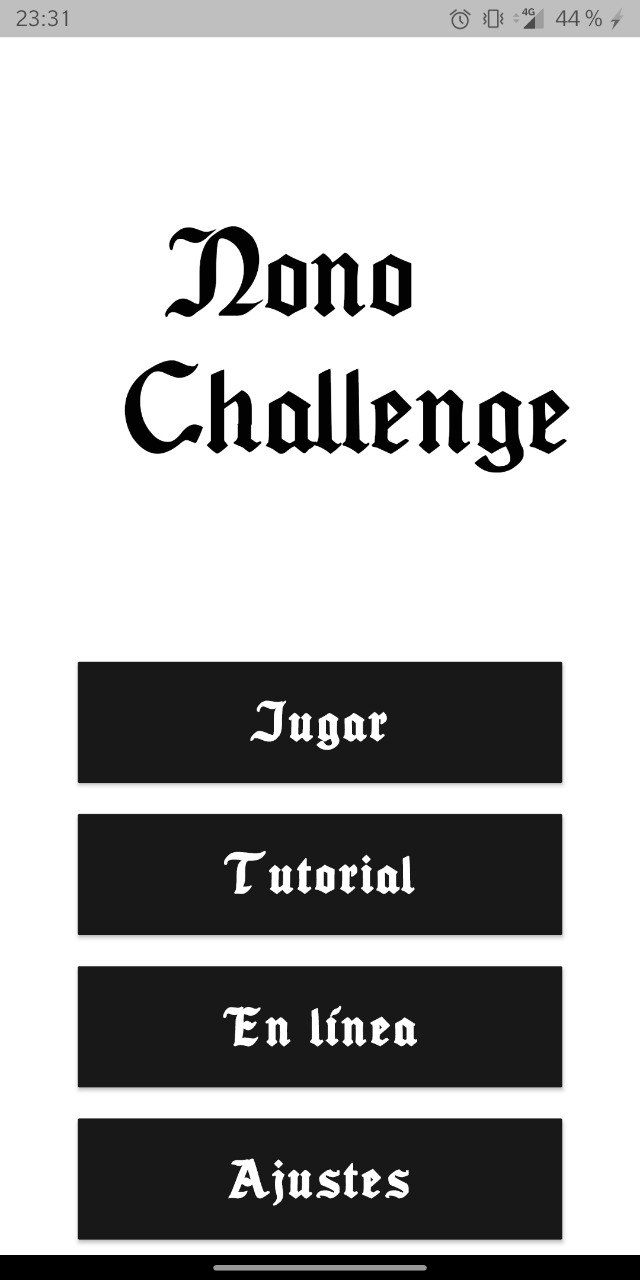
\includegraphics[width=\linewidth]{images/man1.jpeg}
      \caption{Pantalla inicio}
      \label{fig:man1-1}
    \end{subfigure}
    \begin{subfigure}[b]{0.36\linewidth}
      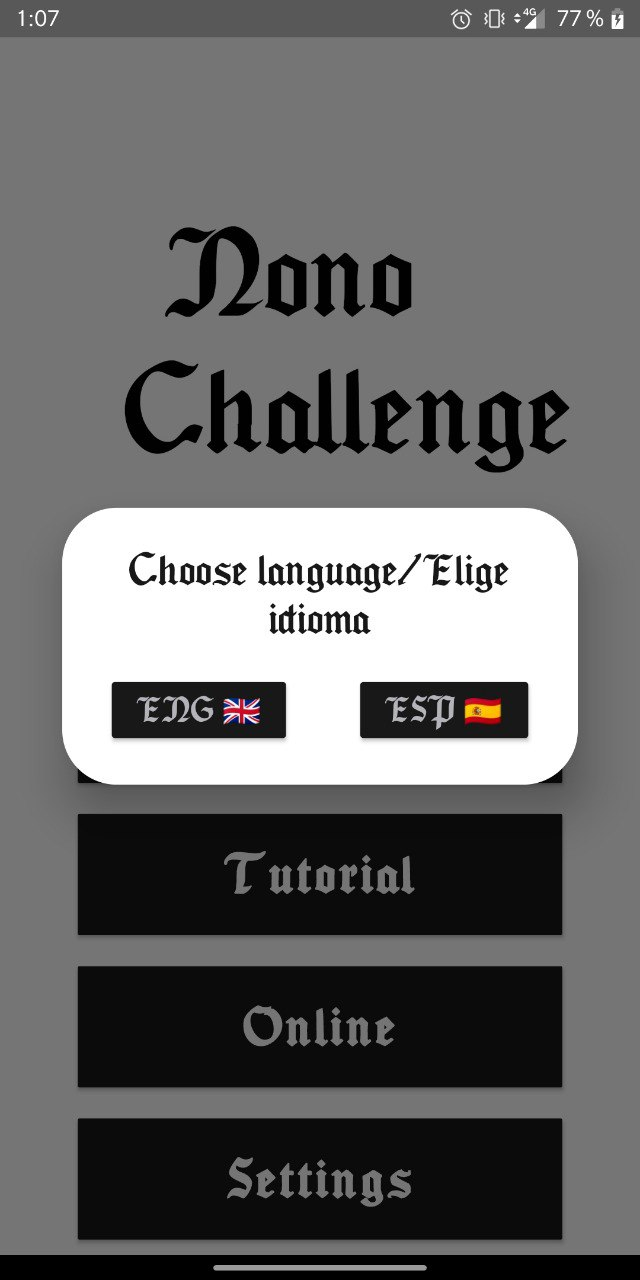
\includegraphics[width=\linewidth]{images/man2.jpeg}
      \caption{Pop-up selector de idioma}
      \label{fig:man1-2}
    \end{subfigure}
    \caption{Pantallas iniciales}
    \label{fig:man1}
  \end{figure}

Mediante los botones del menú, el usuario puede ingresar a cada una de las
secciones que lo componen.

\section{Pantalla Jugar nonogramas clásicos}
Dentro del primer menú de \textit{Jugar} encontraremos una lista de niveles
predefinidos, muchos de ellos son niveles tradicionales extraídos de los publicados por
el noticiario \textit{The Sunday Telegraph}.
En cuanto se resuelve un \textit{nonograma}, se descubre el nombre del
nivel, que representa la figura del \textit{nonograma} resuelto.

El sistema presenta autoguardado que, en el caso de estar activado en \textit{Ajustes},
da la opción de volver al nivel justo en el punto donde lo dejaste por última vez.

Esta característica, como se había comentado anteriormente en el análisis de requisitos es
un imprescindible, ya que es muy recurrente en este tipo de pasatiempos, sobre todo
en la resolución de niveles grandes dimensiones.

En el caso de no seleccionar la opción de cargado, por cualquiera de estas
casuísticas, la resolución del \textit{nonograma} estará completamente
nuevo con un progreso inexistente.

\begin{figure}[H]
    \centering
    \begin{subfigure}[b]{0.45\linewidth}
      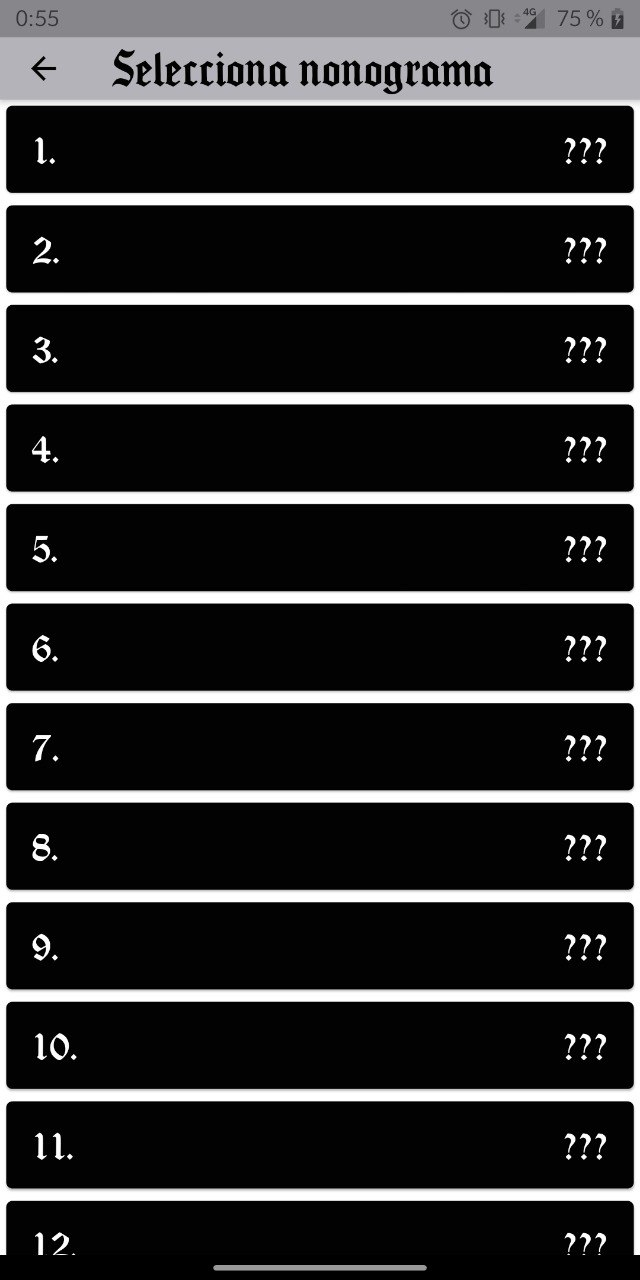
\includegraphics[width=\linewidth]{images/man3.jpeg}
      \caption{Pantalla selector de nivel}
      \label{fig:man1-3}
    \end{subfigure}
    \begin{subfigure}[b]{0.45\linewidth}
      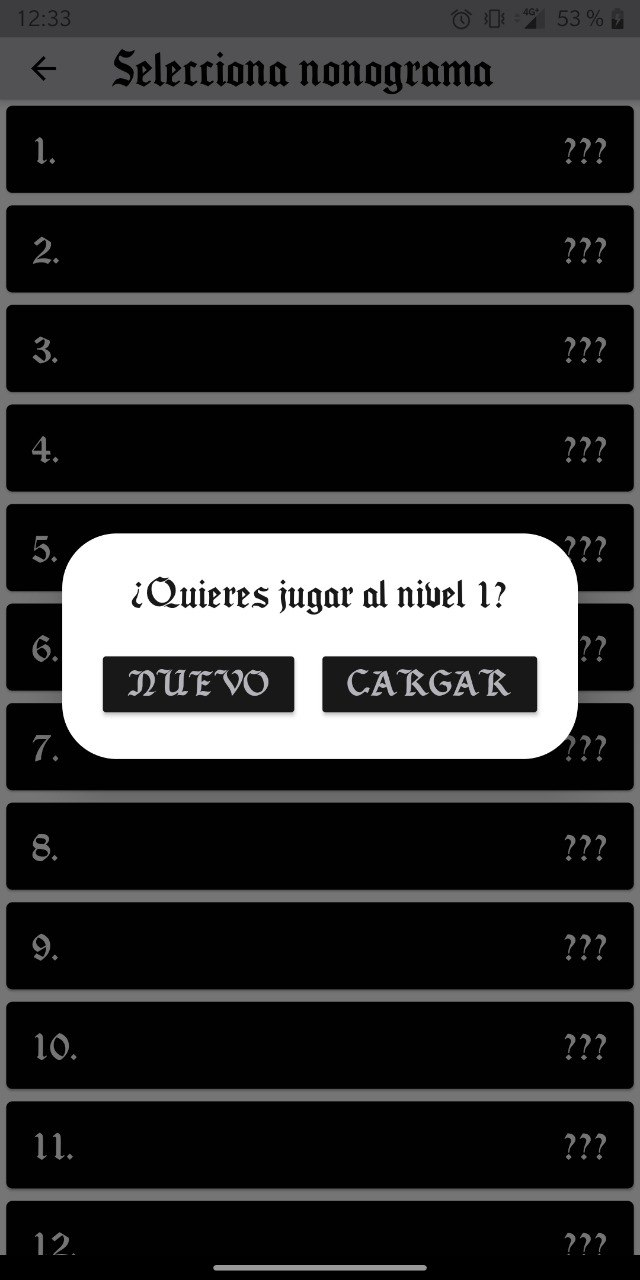
\includegraphics[width=\linewidth]{images/man4.jpeg}
      \caption{Pop-up cargar nivel}
      \label{fig:man1-4}
    \end{subfigure}
    \caption{Pop-up cargar nivel}
    \label{fig:man2}
  \end{figure}

  \section{Pantalla Tutorial}
La pantalla de tutorial, explica de forma sencilla el uso del aplicativo,
además de presentar las bases y consejos para la resolución de \textit{nonogramas}.
El usuario podrá manejarse por cada una de las páginas deslizando hacia izquierda
y derecha la información en el idioma establecido.

\begin{figure}[H]
    \centering
    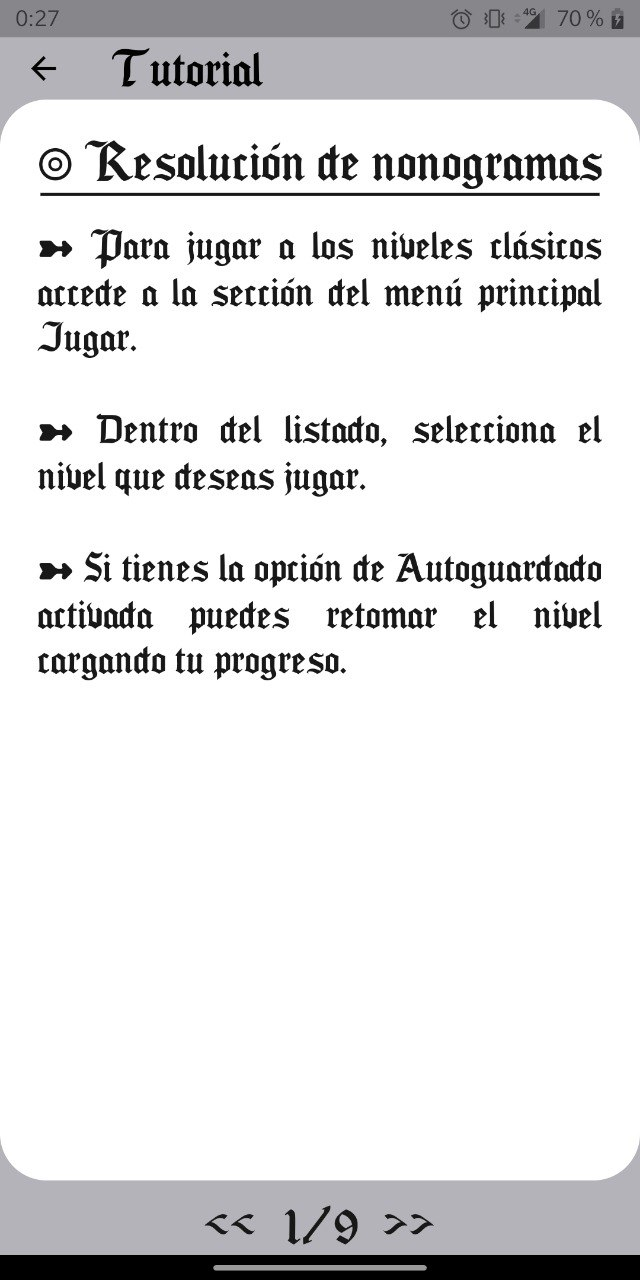
\includegraphics[scale=.3]{images/man5.jpeg}
    \caption{Pantalla de tutorial}
    \label{fig:man3}
  \end{figure}

  \section{Pantalla Resolución de nivel}
  Esta es una de las pantallas principales del aplicativo. Esta, como
  su nombre indica, permite tanto, la resolución de los niveles clásicos, como
  los de en línea creados por otros usuarios. 
  
  Como en los \textit{nonogramas}
  de los medios tradicionales, las matrices de celdas presentan etiquetas en la fila y columna externas,
  indicando el número de celdas correctas divididas en bloques que hay en cada fila o columna.
  Una vez que se van resolviendo las etiquetas van disminuyendo su opacidad indicando su
  resolución.

  El usuario puede seleccionar la celdas correctas haciendo un simple clic sobre ellas.
  De forma similar, se puede realizar doble clic o mantener pulsado las celdas, marcando o desmarcando
  con un aspa las celdas, para indicar
  que esas celdas pueden ser incorrectas y evitar hacer clic sobre ellas.

  Una característica realmente útil, sobre todo para los niveles de mayor dimensiones, tales como el 10x10 de la \autoref{fig:man4},
  el usuario puede acercar o alejar la vista para evitar pulsar una
  celda equivocada. En este modo, se muestra de forma persistente en la barra superior principal, el número de
  vidas que dispone el jugador en todo momento.

  \begin{figure}[H]
    \centering
    \begin{subfigure}[b]{0.45\linewidth}
      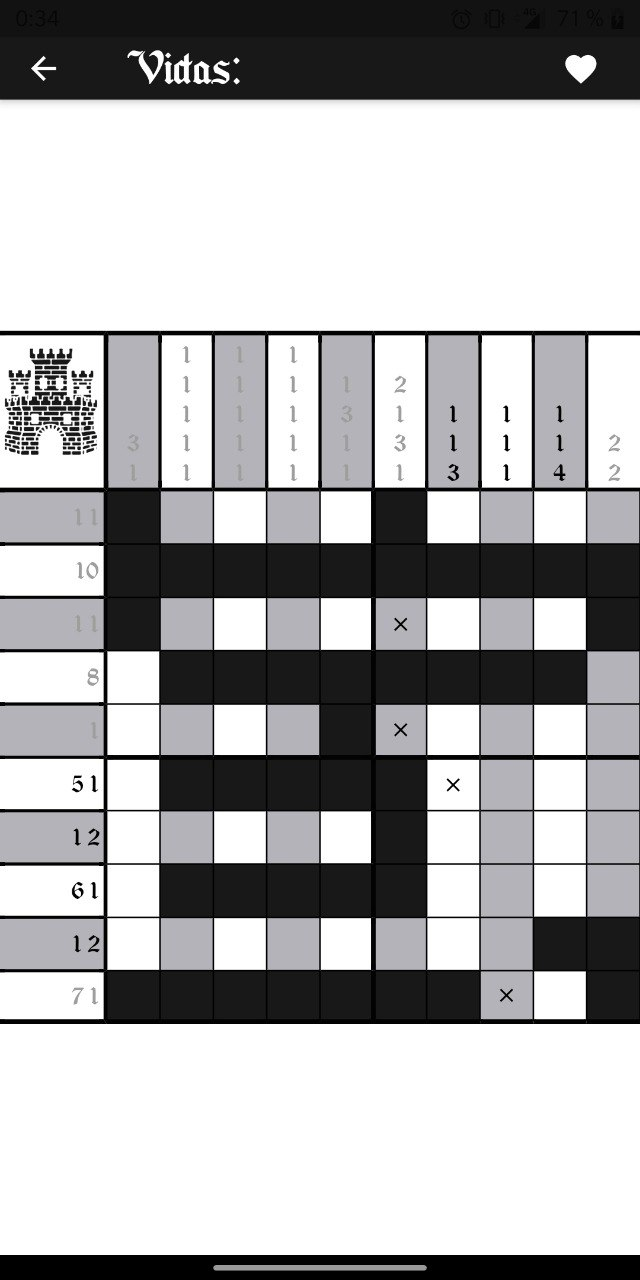
\includegraphics[width=\linewidth]{images/man6.jpeg}
      \caption{Nivel 15x15}
      \label{fig:man1-6}
    \end{subfigure}
    \begin{subfigure}[b]{0.45\linewidth}
      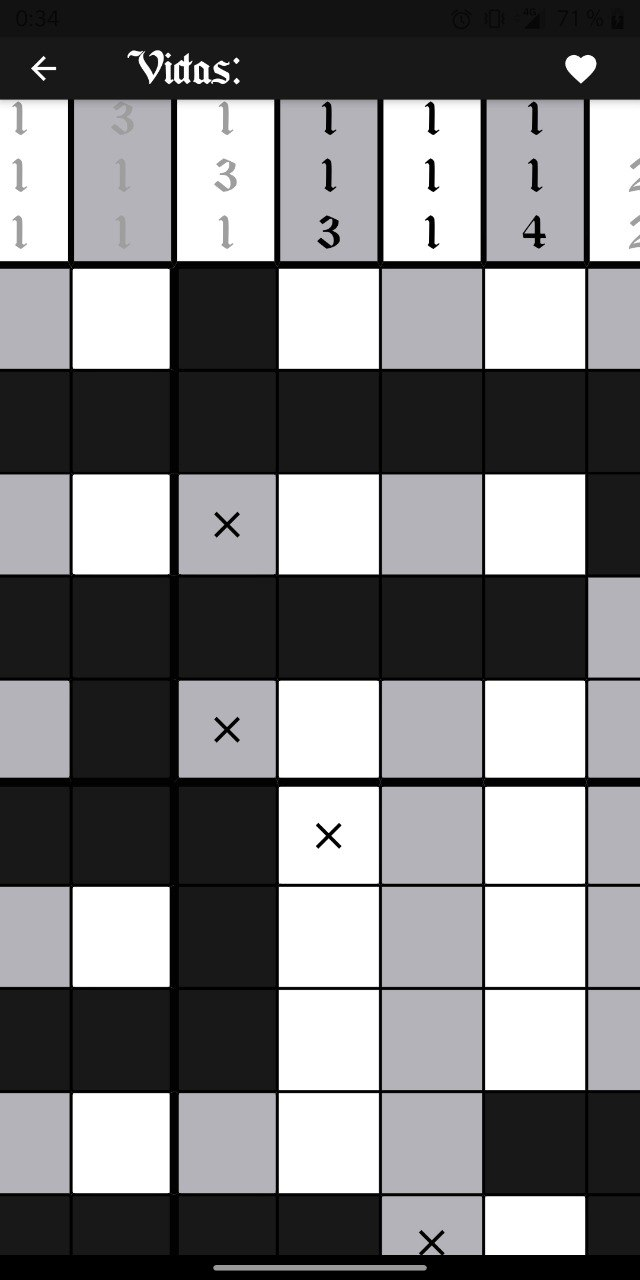
\includegraphics[width=\linewidth]{images/man7.jpeg}
      \caption{Nivel 15x15 con zoom}
      \label{fig:man1-7}
    \end{subfigure}
    \caption{Pantalla resolución de nivel}
    \label{fig:man4}
  \end{figure}

  \section{Pantallas En línea}
  Estas pantallas corresponden, como su nombre indica, a las pantallas
  relacionadas con funciones \textit{en línea}. Para hacer uso de las
  siguientes funcionalidades el dispositivo debe de disponer de conexión
  a Internet.

  Una vez se accede a la sección \textit{En línea}, el usuario puede visualizar
  todos los \textit{nonogramas} publicados de la comunidad, dispuestos en
  celdas, cada uno de ellos está representado por su nombre, figura y autor.

  Para poder crear niveles y publicarlos para la comunidad se presionará
  el botón flotante, situado en el borde inferior izquierdo. El siguiente
  paso es rellenar las características y dimensiones del mismo. Finalmente,
  desde la pantalla de \textit{Creación de nonograma}, decidir las celdas
  correctas, ``dibujando'' y formando el \textit{nonograma} a publicar, cuando
  ya esté decidido el diseño presionar el botón de Aceptar (\autoref{fig:man1-9}).


  \begin{figure}[H]
    \centering
    \begin{subfigure}[b]{0.45\linewidth}
      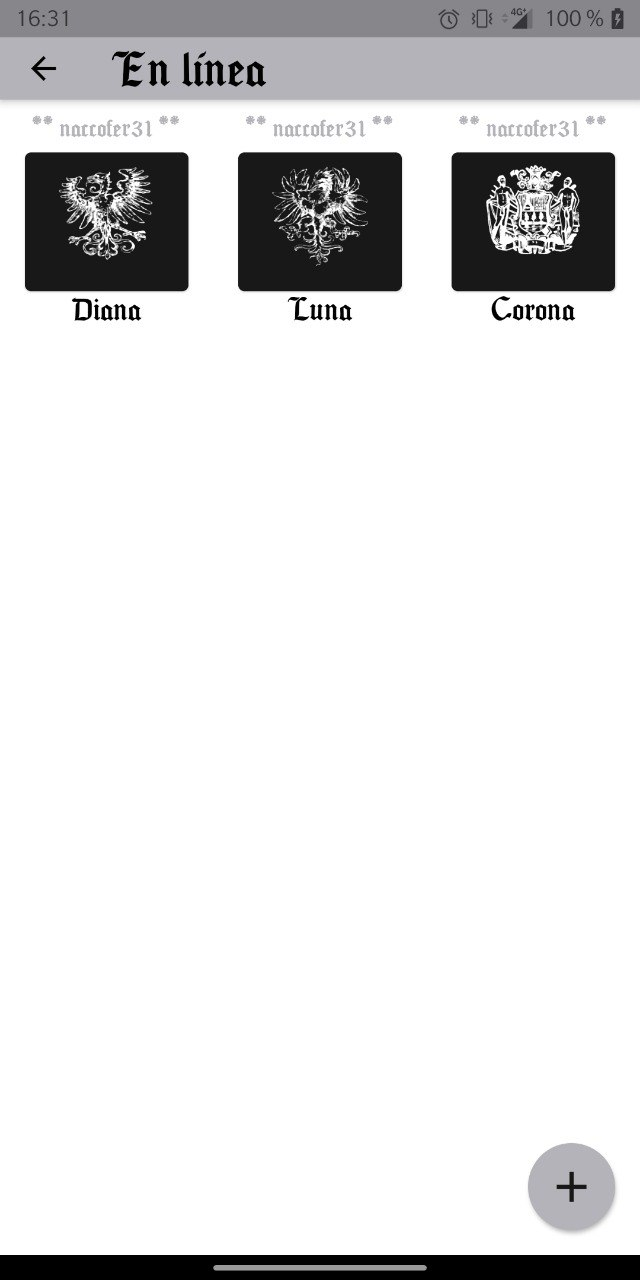
\includegraphics[width=\linewidth]{images/man8.jpeg}
      \caption{Pantalla En Línea}
      \label{fig:man1-8}
    \end{subfigure}
    \begin{subfigure}[b]{0.45\linewidth}
      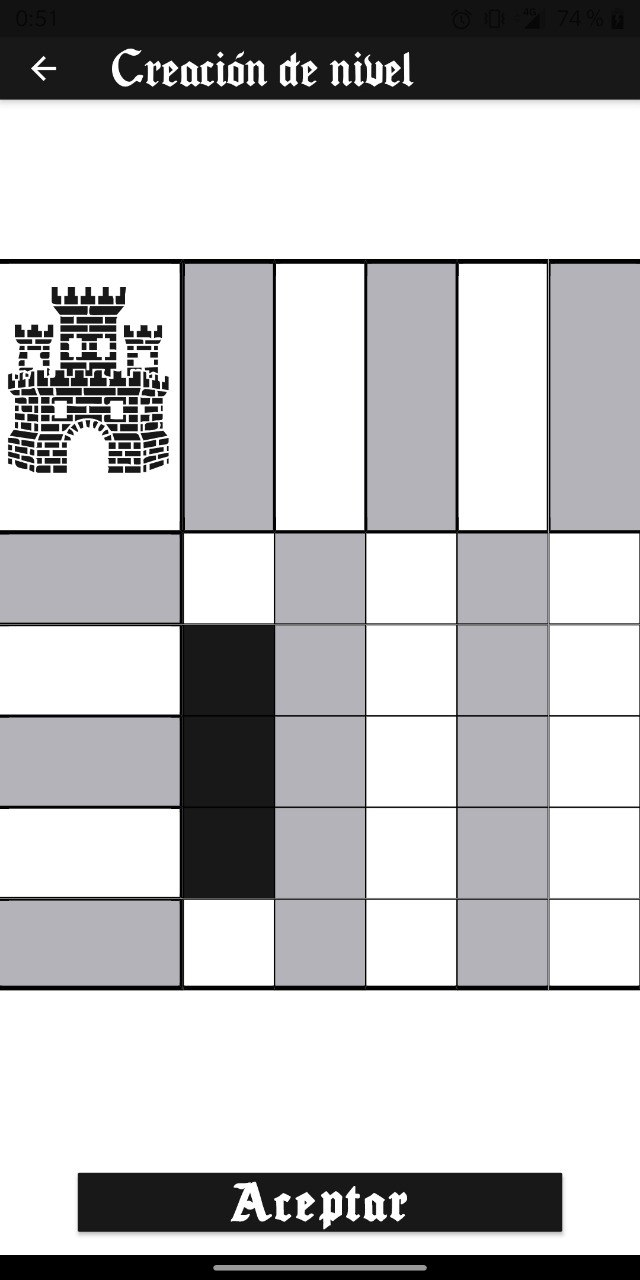
\includegraphics[width=\linewidth]{images/man9.jpeg}
      \caption{Pantalla Creación de nivel}
      \label{fig:man1-9}
    \end{subfigure}
    \caption{Pantalla de funciones En Línea}
    \label{fig:man5}
  \end{figure}

  \section{Pantallas de Ajustes}
  En estas pantallas se ajustan las diferentes configuraciones del sistema,
  ya comentadas anteriormente como: el número de vidas en partida, el idioma y
  opción de autoguardado.

  La penúltima opción del listado de ajustes
  permite acceder a la pantalla de sincronización, en la que el usuario
  puede iniciar sesión mediante \textit{Google} para cargar su progreso tanto
  en niveles clásicos como en línea, además de permitir publicar \textit{nonogramas}
  para la comunidad.

  La última opción de ``Borrar progreso'' permite, como su nombre indica, borrar
  de forma interna, todos los progresos que se hayan guardado en la base de datos
  local del dispositivo.

  Por último, el aplicativo también dispone de un selector de temas de diseño (Tema) que cambian
  a nivel global la paleta de colores del aplicativo (\autoref{fig:man7}). Estos
  están compuestos de un nombre y tres colores diferenciados, que combinados,
  cambian el aspecto completo del aplicativo.
  
  \begin{figure}[H]
    \centering
    \begin{subfigure}[b]{0.4\linewidth}
      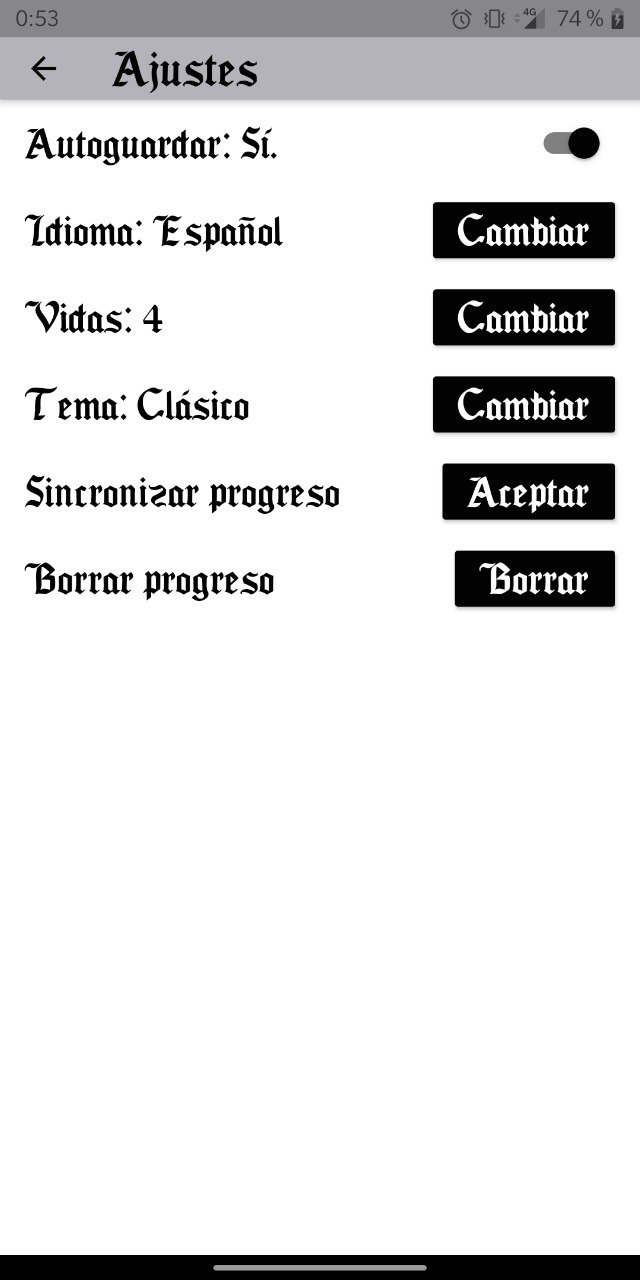
\includegraphics[width=\linewidth]{images/man10.jpeg}
      \caption{Pantalla de Ajustes}
      \label{fig:man1-10}
    \end{subfigure}
    \begin{subfigure}[b]{0.4\linewidth}
      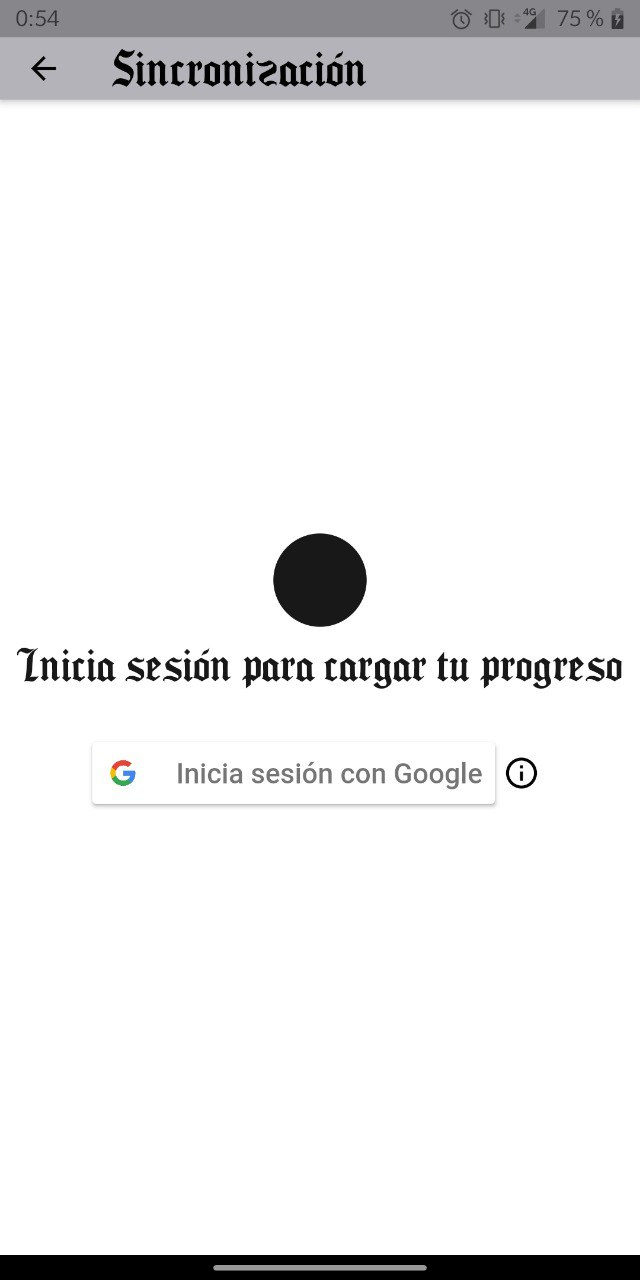
\includegraphics[width=\linewidth]{images/man11.jpeg}
      \caption{Pantalla de sincronización}
      \label{fig:man1-11}
    \end{subfigure}
    \caption{Pantallas de Ajustes}
    \label{fig:man6}
  \end{figure}

  \begin{figure}[H]
    \centering
    \begin{subfigure}[b]{0.22\linewidth}
      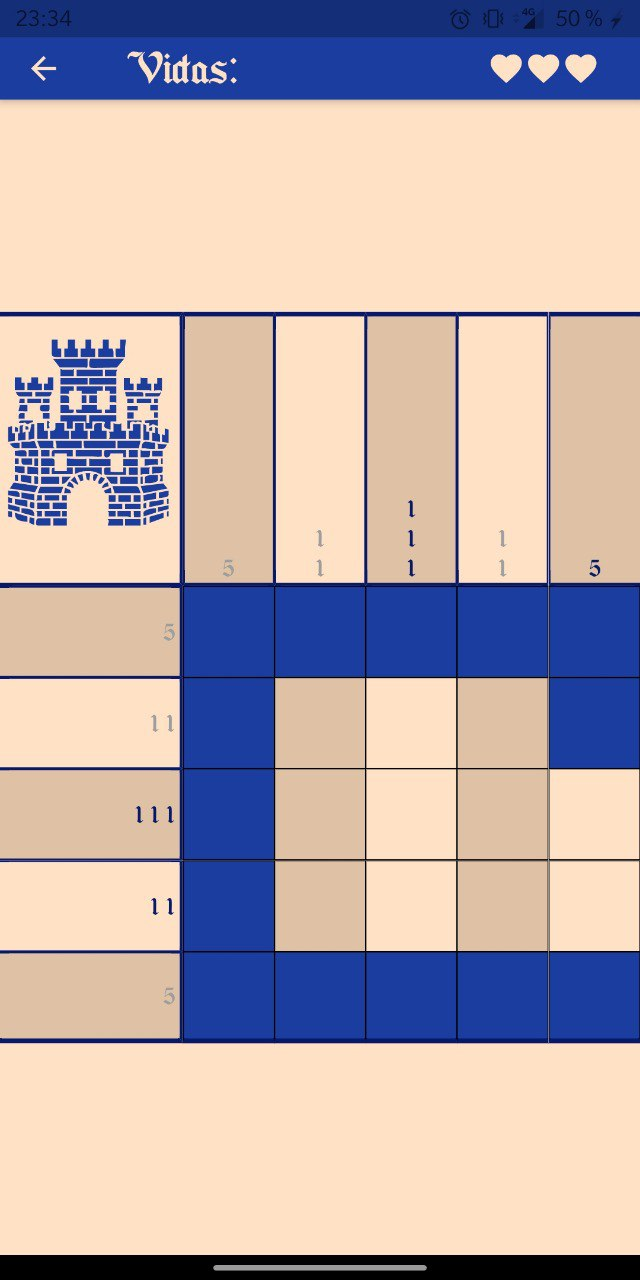
\includegraphics[width=\linewidth]{images/man12.jpeg}
    \end{subfigure}
    \begin{subfigure}[b]{0.22\linewidth}
      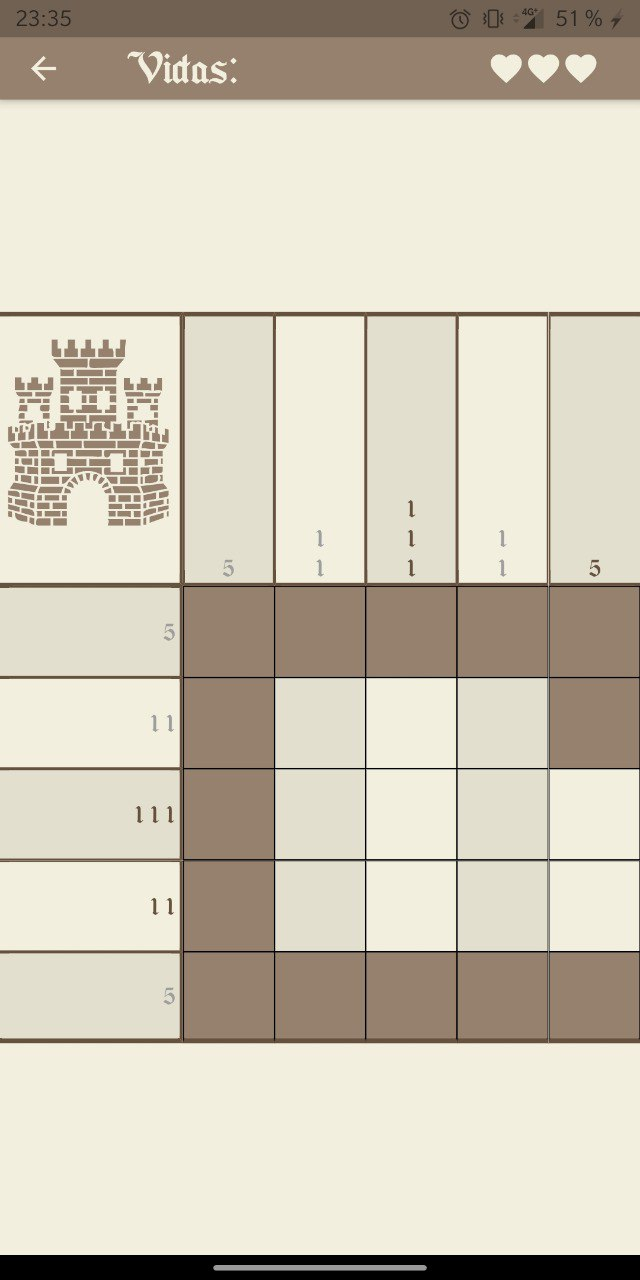
\includegraphics[width=\linewidth]{images/man13.jpeg}
    \end{subfigure}
    \begin{subfigure}[b]{0.22\linewidth}
        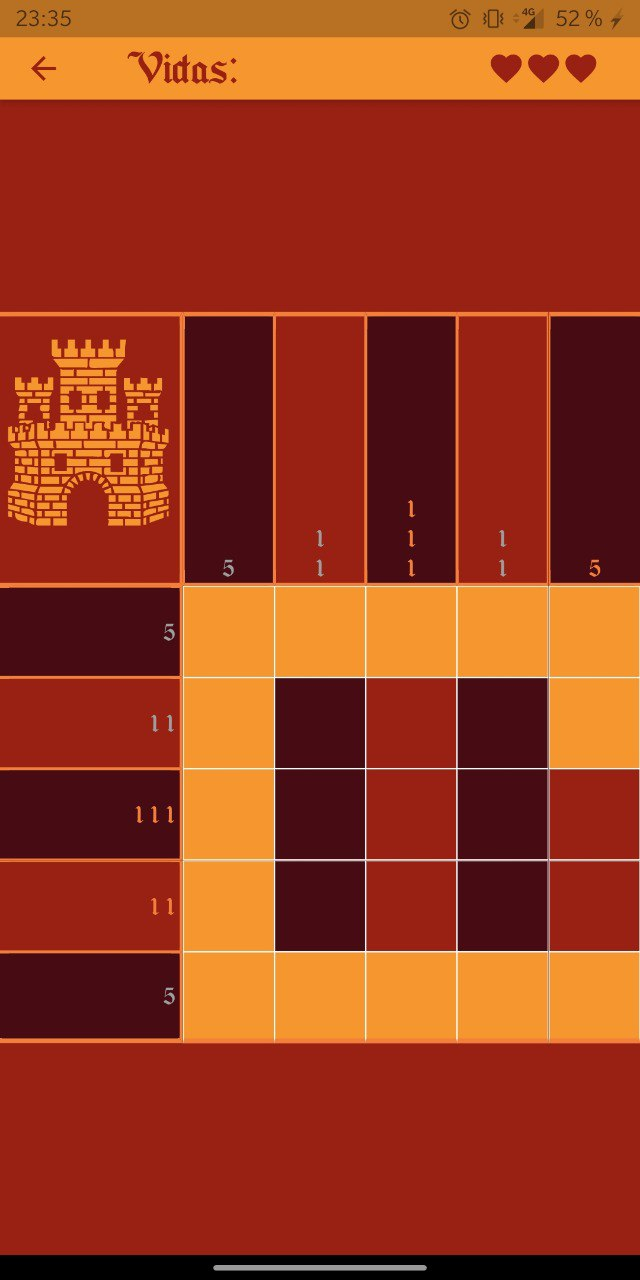
\includegraphics[width=\linewidth]{images/man14.jpeg}
      \end{subfigure}
    \begin{subfigure}[b]{0.22\linewidth}
        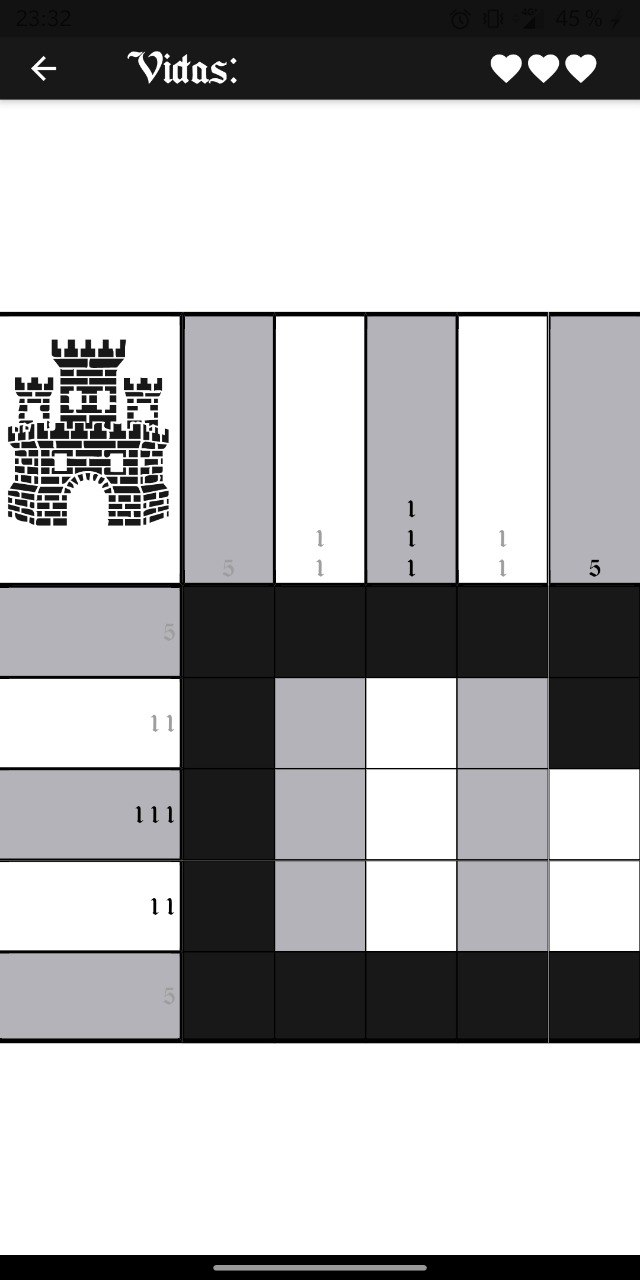
\includegraphics[width=\linewidth]{images/man15.jpeg}
      \end{subfigure}
    \caption{Temas visuales globales del aplicativo}
    \label{fig:man7}
  \end{figure}